\documentclass{article}
\input{structure.tex} % Include the file specifying the document structure and custom commands

% ----------------------------------------------------------------------------------------
% TITOLO
% ----------------------------------------------------------------------------------------
\title{Generic Title}
\author{Mario Giordano \\ \texttt{mario.giordano@pietropacciani.it}}
\date{Università di Firenze --- \today}

% ----------------------------------------------------------------------------------------
\begin{document}


\maketitle

\section*{Introduzione}
Lorem ipsum dolor sit amet consectetur adipiscing elit. Quisque faucibus ex sapien vitae pellentesque sem placerat. 

% TAVOLA DEI CONTENUTI
\tableofcontents
\newpage


\section{Section 1}
\subsection{Subsection 1.1}
Lorem ipsum dolor sit amet consectetur adipiscing elit.

\begin{equation}
Pietro = Pacciani \implies E = mc^2
\end{equation}

\subsection{Subsection 1.2}
\begin{lstlisting}[language=C]
#include <stdio.h>
#include <stdlib.h>

int main(int argc, char ** argv){
    printf("Ritorneremo prima o dopo!\n");
    return 0;
}
\end{lstlisting}

\begin{commandline}
\begin{verbatim}
$ gcc pacciani.c -o pacciani.exe
$ ./pacciani.exe se nimmondo... 
eistesse un po di bene
\end{verbatim}
\end{commandline}

\begin{center}
\begin{minipage}{0.5\linewidth}
\begin{algorithm}[H]
\KwIn{$A$, array di n pietro pacciani}
A.heap\_size = 1 \;
\For{$i=2$ to A.lenght}{
    MAX\_HEAP\_INSERT(A, A[i])
}
\caption{\texttt{build\_max\_heap\_v2}}
\end{algorithm}
\end{minipage}
\end{center}

\begin{equation}
I = \int_{a}^{b} f(x) \; \text{d}x.
\end{equation}

\begin{info}
Questo è un blocchetto informativo di esempio.
\end{info}

\begin{question}
Quisque ullamcorper placerat ipsum.
\begin{enumerate}[label=\alph*)]
\item Do this.
\item Do that.
\item Do something else.
\end{enumerate}
\end{question}

\begin{center}
\begin{minipage}{0.5\linewidth}
\begin{algorithm}[H]
\KwIn{$(a, b)$, due numeri floating-point}
\KwResult{$(c, d)$, tali che $a+b = c+d$}
\If{$|b| > |a|$}{
  scambia $a$ e $b$\;
}
$c \leftarrow a+b$\;
$z \leftarrow c-a$\;
$d \leftarrow b-z$\;
\Return $(c,d)$\;
\caption{\texttt{FastTwoSum}}
\end{algorithm}
\end{minipage}
\end{center}

\begin{question}[\itshape (with optional title)]
Mappa della memoria:

\end{question}
\begin{center}
    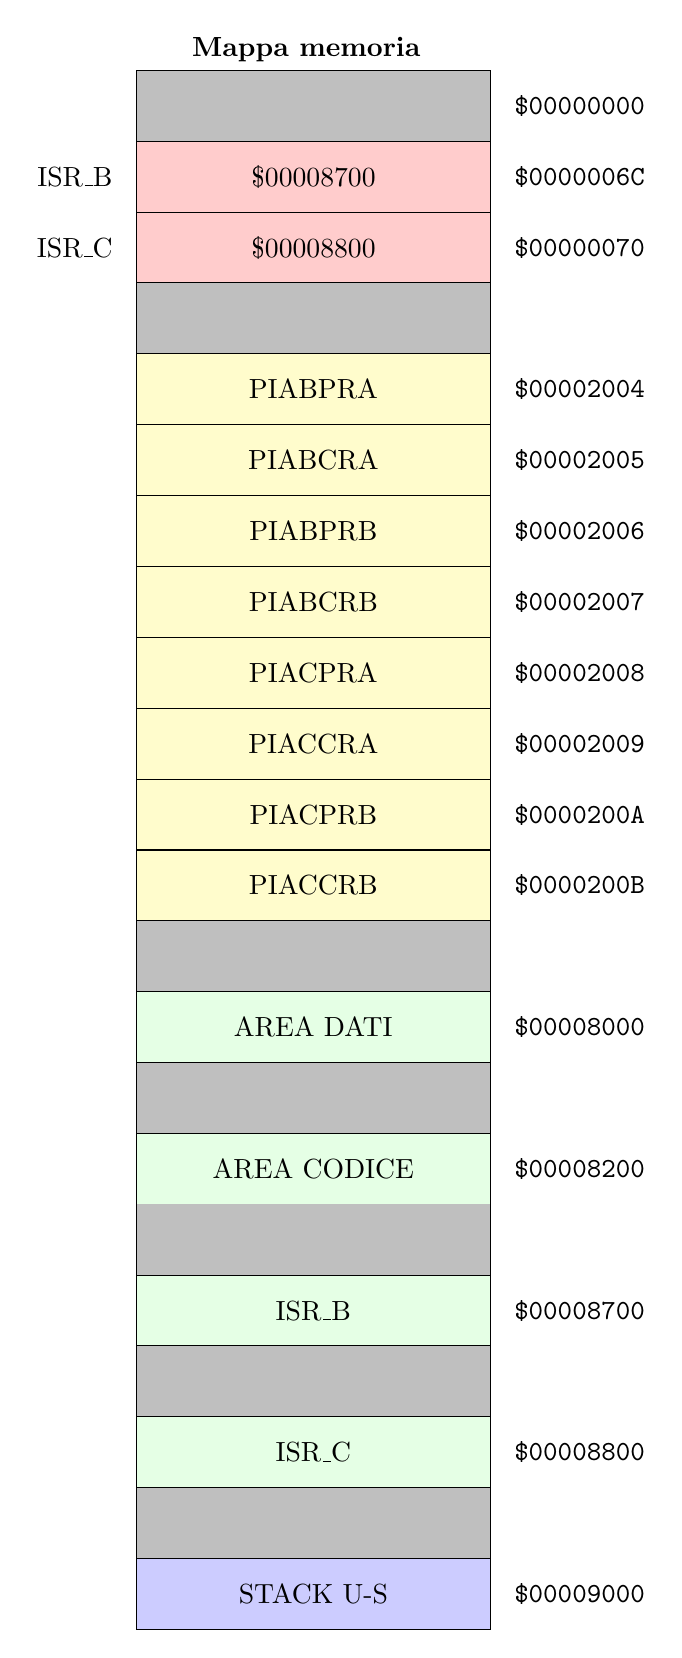
\begin{tikzpicture}[scale=0.9]
        % Rettangolo principale
        \draw (0,0) rectangle (5,20);
        \node at (2.4,20.3) {\textbf{Mappa memoria}};
        
        % vuoto
        \draw (0,20) rectangle (5,19);
        \node[right=5pt] at (5,19.5) {\texttt{\$00000000}};
        \fill[lightgray] (0,20) rectangle (5,19);
        % INT3
        \fill[red!20](0,19) rectangle (5,17);
        \draw (0,19) rectangle (5,18);
        \node[left=5pt] at (0,18.5) {ISR\_B};
        \node[right=5pt] at (5,18.5) {\texttt{\$0000006C}};
        \node at (2.5,18.5) {\$00008700}; 
        
        % INT4 
        \draw (0,18) rectangle (5,17);
        \node[left=5pt] at (0,17.5) {ISR\_C};
        \node[right=5pt] at (5,17.5) {\texttt{\$00000070}};
        \node at (2.5,17.5) {\$00008800};

        % vuoto
        \draw (0,17) rectangle (5,16);
        \fill[lightgray] (0,17) rectangle (5,16);
        %PIA 
        \fill[yellow!20](0,16) rectangle (5,8);
        \draw(0,16) rectangle (5,15);
        \node[right=5pt] at (5,15.5) {\texttt{\$00002004}};
        \node at (2.5,15.5) {PIABPRA};
        \draw(0,15) rectangle (5,14);
        \node[right=5pt] at (5,14.5) {\texttt{\$00002005}};
        \node at (2.5,14.5) {PIABCRA};
        \draw(0,14) rectangle (5,13);
        \node[right=5pt] at (5,13.5) {\texttt{\$00002006}};
        \node at (2.5,13.5) {PIABPRB};
        \draw(0,13) rectangle (5,12);
        \node[right=5pt] at (5,12.5) {\texttt{\$00002007}};
        \node at (2.5,12.5) {PIABCRB};

        \draw(0,12) rectangle (5,11);
        \node[right=5pt] at (5,11.5) {\texttt{\$00002008}};
        \node at (2.5,11.5) {PIACPRA};
        \draw(0,11) rectangle (5,10);
        \node[right=5pt] at (5,10.5) {\texttt{\$00002009}};
        \node at (2.5,10.5) {PIACCRA};
        \draw(0,10) rectangle (5,9);
        \node[right=5pt] at (5,9.5) {\texttt{\$0000200A}};
        \node at (2.5,9.5) {PIACPRB};
        \draw(0,9) rectangle (5,8);
        \node[right=5pt] at (5,8.5) {\texttt{\$0000200B}};
        \node at (2.5,8.5) {PIACCRB};

        % vuoto
        \draw (0,8) rectangle (5,7);
        \fill[lightgray] (0,8) rectangle (5,7);
        
        % DATI
        \fill[green!10] (0,7) rectangle (5,0);
        \draw(0,7) rectangle (5,6);
        \node[right=5pt] at (5,6.5) {\texttt{\$00008000}};
        \node at (2.5,6.5) {AREA DATI};

        
        % vuoto
        \draw (0,6) rectangle (5,5);
        \fill[lightgray] (0,6) rectangle (5,5);
        
        % CODICE
        \draw(0,5) rectangle (5,4);
        \node[right=5pt] at (5,4.5) {\texttt{\$00008200}};
        \node at (2.5,4.5) {AREA CODICE};

        % vuoto
        \draw (0,4) rectangle (5,3);
        \fill[lightgray] (0,4) rectangle (5,3);

        % ISRB 
        \draw(0,3) rectangle (5,2);
        \node[right=5pt] at (5,2.5) {\texttt{\$00008700}};
        \node at (2.5,2.5) {ISR\_B};

        % vuoto
        \draw (0,2) rectangle (5,1);
        \fill[lightgray] (0,2) rectangle (5,1);

        % ISRC
        \draw(0,1) rectangle (5,0);
        \node[right=5pt] at (5,0.5) {\texttt{\$00008800}};
        \node at (2.5,0.5) {ISR\_C};

        % vuoto 
        \draw(0,0) rectangle (5,-1);
        \fill[lightgray](0,0) rectangle (5,-1);
        % STACK
        \fill[blue!20](0,-1) rectangle (5,-2);
        \draw (0,-1) rectangle (5,-2);
        \node[right=5pt] at (5,-1.5) {\texttt{\$00009000}};
        \node at (2.5,-1.5) {STACK U-S};

        \draw(0,-2) rectangle (5,20); % ricalco bordi
    \end{tikzpicture}
\end{center}



% Tabella descrittiva
\begin{description}[style=nextline,leftmargin=3.45cm,labelwidth=2.8cm,labelsep=0.6cm,font=\ttfamily\bfseries]
\item[esempio1] Intero che può assumere i valori 0 o 1.
\item[esempio2] Intero che può assumere i valori 0 o 1.
\end{description}

% \begin{lstlisting}
% c code snippet
% \end{lstlisting}

% \begin{lstlisting}[language={[x86masm]Assembler}]
% asm code snippet
% \end{lstlisting}

\begin{warn}[Osservazione:]
Questo è un messaggio di warning.
\end{warn}

\end{document}